\chapter{Phương pháp để xuất}
% Trình bày chi tiết về ý tưởng, các mô hình toán, các chứng minh nếu có. Đồng thời trình bày các bước thực hiện và khảo sát, kiểm nghiệm kết quả nghiên cứu. Mô tả kết quả nghiên cứu khi thử nghiệm với nhiều tập dữ liệu và những độ khó khác nhau.

\section{Ý tưởng thực hiện luận văn}

Nhắc lại yêu cầu bài toán: Tạo sinh video khuôn mặt người đang nói dựa trên một hình ảnh tĩnh chứa mặt người mẫu và một đoạn âm thanh chứa tiếng nói. Qua yêu cầu bài toán ta thấy, đầu vào của hệ thống có tính chất khác với đầu ra, sử dụng hình ảnh tĩnh và âm thanh để tạo ra hình ảnh chuyển động. Một số yêu cầu quan trọng khác quyết định chất lượng của chuỗi hình ảnh được tạo sinh ra cũng cần được chú ý. Đó là:
\begin{itemize}
    \item Hình ảnh phải chân thật, rõ ràng, thể hiện được đúng hình dáng gương mặt người đang nói, không bị méo mó, dị dạng.
    \item Chuỗi hình ảnh được tạo sinh cần phải giữ được đặc trưng gương mặt trong ảnh mẫu. Có nghĩa là, người xem vẫn có thể nhận ra được mặt người đang nói trong video được tạo sinh chính là người trong hình ảnh ban đầu
    \item Khẩu hình miệng khi chuyển động phải khớp với âm thanh được nói ra. Sự chuyển động của môi và miệng trong video được tạo sinh phải thể hiện được cách phát âm từ được nói gần như trong thực tế
\end{itemize}

Dựa theo yêu cầu bài toán, ta cần tìm kiếm một phương pháp để kết hợp đặc trưng âm thanh và hình ảnh lại với nhau, sau đó chuyển đổi đặc trưng này thành video. Để mang lại sự trung thực, sắc nét cho hình ảnh được tạo sinh cũng như lưu giữ được các đặc trưng khuôn mặt người trong hình ảnh ban đầu, chiến thuật của ta là sẽ dựa hoàn toàn trên hình ảnh ban đầu để tạo sinh các khung hình khác trong video. Như vậy, với mỗi khung hình ở mỗi thời điểm $t$ trên video, ta cần phải tìm kiếm sự thay đổi của khung ảnh tại thời điểm đó so với hình ảnh tĩnh được cho ban đầu. Sau đó, ta thực hiện biến đổi hình ảnh được cho ban đầu thành hình ảnh ở khung hình tại thời điểm $t$. Như vậy, câu hỏi đặt ra là ta cần phải thay đổi tại vùng nào trên ảnh mẫu và tại những vùng đó ta sẽ thay đổi như thế nào, thay đổi nhiều hay ít.

Sự thay đổi của hình ảnh được quyết định phần nhiều bởi chuỗi âm thanh được đưa vào hệ thống. Âm thanh giọng nói quyết định khẩu hình miệng và các biểu cảm trên gương mặt, đôi khi còn có thể quyết định cách chuyển động của đầu. Tuy giọng nói góp phần lớn khi định hình sự thay đổi trên gương mặt, ảnh mẫu ban đầu cũng quyết định phần nào các thay đổi đó. Hình ảnh ban đầu cung cấp thông tin về nhận dạng khuôn mặt, về những đặc điểm của các bộ phận trên gương mặt người nói, về vị trí của mắt, mũi, miệng để định hình cách âm thanh thay đổi hình dạng gương mặt.

\begin{figure}[H]
    \centering
    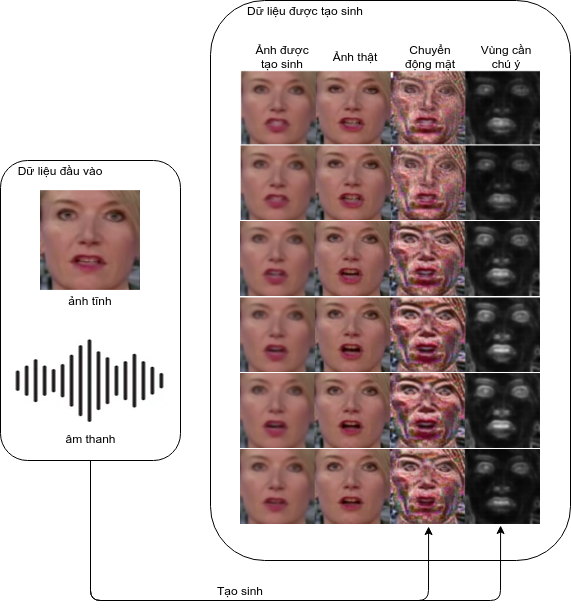
\includegraphics[width=12cm]{./content/materials/idea.png}
    \caption{Ý tưởng về tạo sinh chuỗi hình ảnh chuyển động cho mặt người đang nói}
\end{figure}

Ý tưởng giải quyết bài toán được thể hiện ở hình trên. Chúng ta sẽ tạo ra một hệ thống có khả năng trích xuất đặc trưng của hình ảnh tĩnh ban đầu và âm thanh giọng nói để tạo ra hình ảnh chuyển động của mặt. Tuy nhiên, hình ảnh chuyển động mặt này không hoàn toàn được sử dụng, mà song song với nó, ta tạo ra một mặt nạ tương ứng. Mặt nạ này chỉ chú ý tới một số khu vực trên hình ảnh chuyển động mặt được tạo sinh. Những vùng màu đen là những vùng không được chú ý đến trên ảnh chuyển động vừa được sinh ra, ngược lại, các vùng có màu trắng càng sáng thì càng được chú ý. Như vậy, mặt nạ chú ý sẽ cho ta biết ta nên thay đổi những vùng nào trên gương mặt tại thời điểm $t$ tương ứng với tiếng nói ở thời điểm đó. Đồng thời, hình ảnh chuyển động mặt được tạo sinh song song cho ta biết ta phải thay đổi như thế nào ở những điểm được chú ý. Ở những điểm không được chú ý còn lại, ta sẽ thay thế bằng các điểm ảnh trong ảnh gốc ban đầu. Nhờ vậy, ta có thể bảo toàn được nhận dạng của người nói trong quá trình tạo sinh bằng việc chỉ tìm ra những điểm thay đổi trên gương mặt thay vì cố gắng tìm cách tạo sinh toàn bộ gương mặt của người nói.

\section{Mô hình hóa bài toán}\label{sec:modeling}

Như phân tích ở phần trên, âm thanh sẽ đóng góp phần lớn vào việc tạo sinh chuyển động cho khuôn mặt. Tuy nhiên, ta thấy dữ liệu dạng sóng biên độ - thời gian của âm thanh dường như không có mối liên hệ tốt với chuyển động trên gương mặt. Vì thế, ta cần xử lý âm thanh để tạo ra một đặc trưng gần gũi hơn với những chuyển động tương ứng trên gương mặt. Đây là một bước cần thiết để hình ảnh được tạo sinh có chất lượng tốt và có được những chuyển động chính xác. Do đó, ta sẽ chuyển âm thanh thành một dạng thể hiện khác, đó là các cột mốc trên gương mặt (Facial Landmark). Cột mốc trên mặt gồm 68 điểm trên không gian hai chiều, mỗi điểm đánh dấu một vị trí trên gương mặt, hình sau cho là ví dụ về cột mốc trên gương mặt người:

\begin{figure}[H]
    \centering
    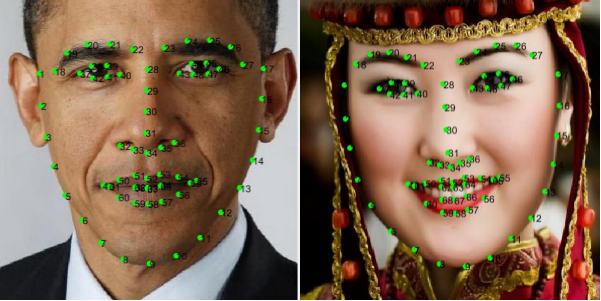
\includegraphics[width=10cm]{./content/materials/landmark_intro.png}
    \caption{Các điểm cột mốc trên khuôn mặt. Hình ảnh được lấy từ bài báo \cite{landmark}}
\end{figure}

Như vậy, từ đoạn âm thanh có chứa tiếng nói và hình ảnh ban đầu, ta sẽ tạo sinh ra một chuỗi cột mốc khuôn mặt để thay thế cho âm thanh làm căn cứ cho những chuyển động trên gương mặt. Cấu trúc tổng quát của hệ thống được thế hiện ở Hình \ref{fig:common_architecture}.

\begin{figure}[H]
    \centering
    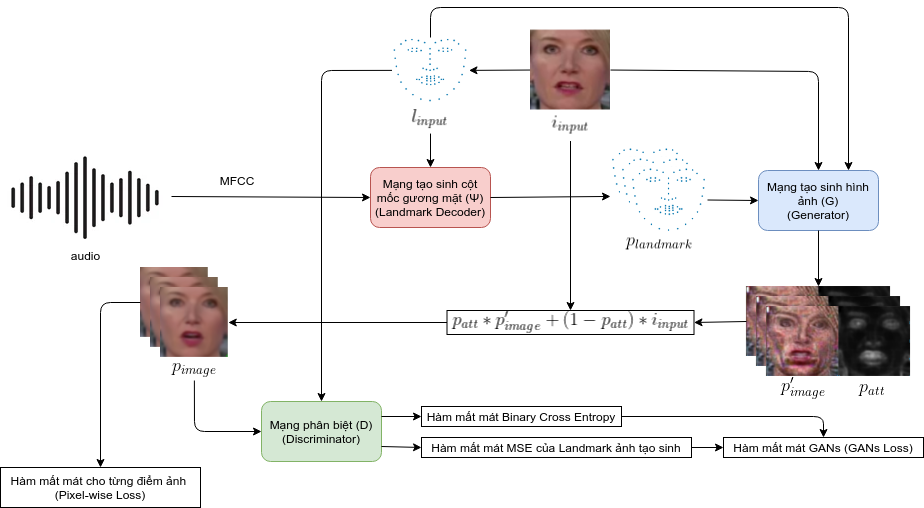
\includegraphics[width=15cm]{./content/materials/common_architecture.png}
    \caption{Cấu trúc tổng quát của hệ thống}
    \label{fig:common_architecture}
\end{figure}

Theo như kiến trúc được thể hiện ở Hình \ref{fig:common_architecture}, hệ thống sẽ trích xuất đặc trưng cột mốc $l_{input}$ trên gương mặt trong hình mẫu $i_{input}$. Sau đó, đặc trưng MFCC sẽ được trích xuất từ âm thanh đầu vào. Đặc trưng MFCC và $l_{input}$ sẽ được đưa vào mạng tạo sinh cột mốc gương mặt (Landmark Decoder). Mạng này kết hợp hai đặc trưng trên với nhau để dự đoán chuỗi các cột mốc gương mặt người khi nói đoạn âm thanh được đưa vào hệ thống ($p_{landmark}$). Từ thời điểm này, âm thanh không còn được sử dụng để tạo sinh hình ảnh mặt người, chuỗi những điểm cột mốc gương mặt $p_{landmark}$ sẽ thay thế cho âm thanh trong những bước xử lý tiếp theo. Như vậy, ta đã tách rời được dữ liệu âm thanh so với phần tạo sinh hình ảnh, và cung cấp cho phần mạng phía sau những đặc trưng dễ học hơn, giàu thông tin hữu ích hơn và ít nhiễu hơn. 

Phần tiếp theo trong hệ thống là cặp mạng tạo sinh (Generator) và phân biệt (Discriminator) tạo nên mạng GANs như đã trình bày ở phần \ref{sec:base_knowledge_gans}. Tuy nhiên, đây không phải là mạng GANs truyền thống mà là mạng GANs có điều kiện (Conditional GANs \cite{conditional_gan}). Thay vì tạo sinh dữ liệu bằng một véc tơ được sinh ra ngẫu nhiên theo phân phối chuẩn, mạng GANs có điều kiện dựa vào một điều kiện đầu để tạo sinh dữ liệu. Trong luận văn này, mạng GANs có điều kiện tạo sinh dữ liệu với điều kiện đầu vào là $i_{input}$, $l_{input}$ và $p_{landmark}$ được cho trước.

Bài toán mà mạng tạo sinh phải giải là đối với mỗi khung ảnh được tạo sinh để phù hợp với giọng nói được cho, ta phải thay đổi hình ảnh gốc $i_{input}$ ở những vị trí nào, và tại vị trí đó, ta phải thay đổi nó như thế nào để sinh ra được hình ảnh mới? Mạng tạo sinh hình ảnh với đầu vào là hình ảnh mẫu $i_{input}$, cột mốc của gương mặt trên hình ảnh mẫu $l_{input}$ và chuỗi cột mốc gương mặt vừa được tạo sinh $p_{landmark}$ có chức năng tạo sinh ra hai chuỗi dữ liệu $p_{att}$ và $p'_{image}$ tương ứng để trả lời cho câu hỏi trên. Chuỗi hình ảnh $p_{att}$ và $p'_{image}$ có cùng chiểu dài và kích thước hình ảnh. Chuỗi hình ảnh $p_{att}$ thể hiện những điểm cần thay đổi trên ảnh gốc và mức độ thay đổi tại điểm đó. Chuỗi dữ liệu còn lại là chuỗi $p'_{image}$ thể hiện những thay đổi trên ảnh gốc để phù hợp với tiếng nói trong âm thanh. Chuỗi $p'_{image}$ có cấu trúc hình ảnh là gương mặt người, có sự thay đổi theo trục thời gian tương ứng với những chuyển động trên gương mặt để phù hợp với giọng nói. Tuy nhiên đây không phải là hình ảnh hoàn chỉnh của gương mặt, chỉ một vài chi tiết cần thiết trên chuỗi $p'_{image}$ được lấy ra và ghép vào ảnh gốc $i_{input}$ để tạo ra hình ảnh cuối cùng. Cũng vì vậy, $p'_{image}$ là chuỗi hình ảnh được sinh ra để cho ta biết hình ảnh gốc nên thay đổi như thế nào. 

Cuối cùng, ta cần phải kết hợp hình ảnh ban đầu $i_{image}$ và chuỗi hình ảnh vừa được sinh ra là $p'_{image}$ và $p_{att}$ lại để tạo thành chuỗi hình ảnh hoàn chỉnh $p_{image}$. Có thể gọi $p_{att}$ là một mặt nạ chú ý (attention mask), mặt nạ này có giá trị các điểm ảnh trong khoảng từ 0 đến 1. Với điểm ảnh càng gần về 0, điểm ảnh cùng vị trí trong $i_{input}$ càng được sử dụng nhiều, điểm ảnh cùng vị trí trong $p'_{image}$ càng ít được sử dụng và ngược lại. Công thức tạo thành $p_{image}$ được biểu diễn như sau:

\begin{equation}
    p_{image}=p_{att}*p'_{image}+(1-p_{att})*i_{input}
\end{equation}

Hình ảnh hoàn chỉnh được tạo sinh $p_{image}$ sau đó được đem đi so sánh với chuỗi hình ảnh trong video gốc để tính giá trị mất mát L1. Giá trị mất mát này được lan truyền ngược để cập nhật các trọng số trong mạng tạo sinh. Chuỗi hình ảnh hoàn chỉnh cũng được đưa vào bộ phân biệt (Discriminator) để bộ phân biệt dự đoán xem chuỗi hình ảnh này là ảnh được tạo sinh (chuỗi hình ảnh giả) hay chuỗi hình ảnh này là hình ảnh được lấy từ tập dữ liệu thật, sai sót của bộ phân biệt được biểu diễn bằng hàm Binary Cross Entropy. Đồng thời bộ phân biệt cũng dựa vào chuỗi hình ảnh được đưa vào và cột mốc gương mặt của ảnh mẫu $l_{input}$ để cố gắng sinh ra một chuỗi cột mốc gương mặt tương ứng với chuỗi hình ảnh $p_{image}$ được đưa vào mạng. Chuỗi cột mốc gương mặt vừa được sinh ra này sẽ được so sánh với chuỗi cột mốc gương mặt được rút trích trực tiếp từ chuỗi hình ảnh trong video gốc. Sự sai khác trong hai chuỗi cột mốc gương mặt được tính bằng hàm mất mát Mean Square Error. Điều này có nghĩa, chuỗi hình ảnh được tạo sinh $p_{image}$ phải rút trích được một chuỗi cột mốc gương mặt sao cho giống nhất với chuỗi cột mốc gương mặt trong video gốc. Tổng hợp của giá trị mất mát Mean Square Error và Binary Cross Entropy vừa nêu, ta được hàm mất mát GANs chung của mạng GANs. Giá trị mất mát GANs này được lan truyền ngược để cập nhật trọng số cho cả mạng tạo sinh và mạng phân biệt.

Tóm lại, việc tạo sinh hình ảnh từ đoạn âm thanh $a(t)$, hình ảnh mẫu $i_{input}$ và cột mốc gương mặt $l_{input}$ được biểu diễn dưới dạng công thức toán như sau:

\begin{equation}
    \begin{split}
    p_{landmark}(t) &= \psi(l_{input}, mfcc(a(t)))\\
    p'_{image}(t), p_{att} &= G(i_{input}, l_{input}, p_{landmark})\\
    p_{image} &= p_{att}*p'_{image}+(1-p_{att})*i_{input}
    \end{split}
\end{equation}

\section{Tiền xử lý dữ liệu}

\subsection{Tiền xử lý âm thanh}
Ta có thể thấy, phần âm thanh ta chú ý đến chỉ là tiếng nói của con người và ta mong muốn loại bỏ các tạp âm khác. Khoảng tần số âm thanh mà con người có thể nghe được dao động trong khoảng từ 20Hz đến 20kHz, và theo như phương pháp lấy mẫu Nyquist, để lấy mẫu một tín hiệu có tần số $x$(Hz), thì bộ lấy mẫu phải lấy mẫu ở tần số ít nhất là $2x$(Hz). Như vậy, khi thu âm, để thu được âm thanh mà con người có thể nghe được, người ta phải lấy mẫu ở tần số thấp nhất là 40kHz. Trên thực tế, trong việc ghi âm, người ta thường lấy mẫu ở tần số 44.1kHz. Hình sau miêu tả các bước xử lý âm thanh trong bài nghiên cứu.

\begin{figure}[H]
    \centering
    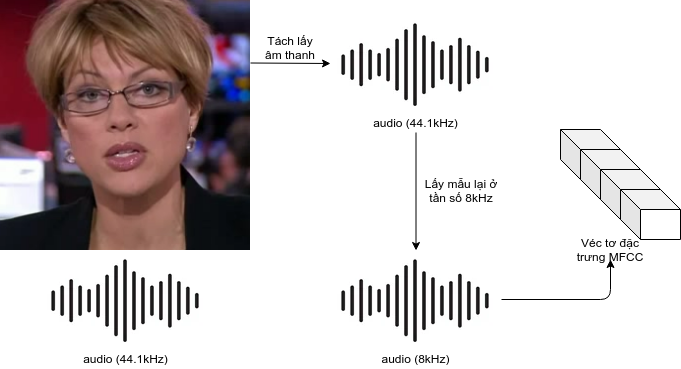
\includegraphics[width=12cm]{./content/materials/preprocess-audio.png}
    \caption{Tiền xử lý tín hiệu âm thanh}
\end{figure}

Tuy nhiên, thanh quản con người chỉ có thể phát ra âm thanh với tần số dưới 4kHz. Vì vậy, để loại bỏ nhiễu ở các dãi tần số cao hơn, ta có thể lấy mẫu lại âm thanh trong video. Theo phương pháp lấy mẫu Nyquist, để lấy được âm thanh có tần số dưới 4kHz, ta cần phải lấy mẫu ở tần số 8kHz. Như vậy, tất cả âm thanh trong tất cả các đoạn video sẽ được lấy mẫu lại ở tần số 8kHz. Bộ lấy mẫu sẽ hoạt động như một bộ lọc thông thấp để loại bỏ nhiễu cao tần trong các đoạn âm thanh. Phương pháp lấy mẫu tần số thấp này cũng được dùng trong các thiết bị thu tiếng nói như máy thu âm, điện thoại để loại bỏ nhiễu.

Âm thanh sau khi lấy mẫu sẽ được đem đi trích xuất để lấy đặc trưng MFCC. Như đã nói ở phần \ref{sec:base_knowledge_mfcc}, MFCC là đặc trưng âm thanh chỉ dành riêng cho tiếng nói của con người. Ta tiến hành lấy đặc trưng MFCC với của sổ trượt 10ms, cứ mỗi cửa sổ trượt 10ms sẽ sinh ra một véc tơ 13 chiều tương ứng với 13 quãng tần số khác nhau, tuy nhiên ta sẽ loại bỏ khoảng tần số đầu do nó có tần số quá thấp và chỉ sử dụng 12 khoảng tần số ở cuối. Như vậy, mỗi cửa sổ 10ms theo trúc thời gian của âm thanh sẽ tạo ra một véc tơ 12 chiều, một đoạn âm thanh sẽ tạo thành một chuôi véc tơ có chiều dài tương ứng với thời gian của nó.

\subsection{Tiền xử lý hình ảnh và trích xuất cột mốc gương mặt}\label{sec:preprocess_audio_lm}

Đầu tiên, tất cả các khung hình của tất cả các video sẽ được nhận diện khuôn mặt bằng mô hình nhận diện khuôn mặt của thư viện Dlib. Từ khung hình đã được nhận diện khuôn mặt này, ta dễ dàng tìm được cột mốc gương mặt trên từng khung hình. Với mỗi cột mốc gương mặt thu được, ta sẽ chuẩn hóa vùng mắt của nó sao cho 2 điểm ngoài của mắt (điểm 37 và 46 trên hình \ref{fig:standard_landmark}(a)) về tọa độ $(0.3, 0.33)$ và $(0.7, 0.33)$ tương ứng. Việc chuẩn hóa này được thực hiện nhờ phép biến đổi tương tự(Similarity Transformation) trên không gian hai chiều, nhờ đó mà tỉ lệ gương mặt gốc không bị thay đổi.

Cột mốc gương mặt chuẩn là cột mốc gương mặt có hình dáng chung chung của mặt người, và không có chứa đặc điểm riêng của gương mặt của bất kì người nào. Như vậy, để tìm ra cột mốc gương mặt chuẩn, ta cần tính giá trị trung bình của một số lượng lớn các cột mốc gương mặt trong các tập dữ liệu hiện có. Cột mốc gương mặt dùng làm chuẩn $l_{standard}$ được tính toán bằng cách lấy trung bình cộng của tất cả những cột mốc gương mặt đã được chuẩn hóa phần mắt như đã miêu tả ở trên.

\begin{figure}[H]
    \centering
    \subfloat[Cột mốc gương mặt đánh số]{{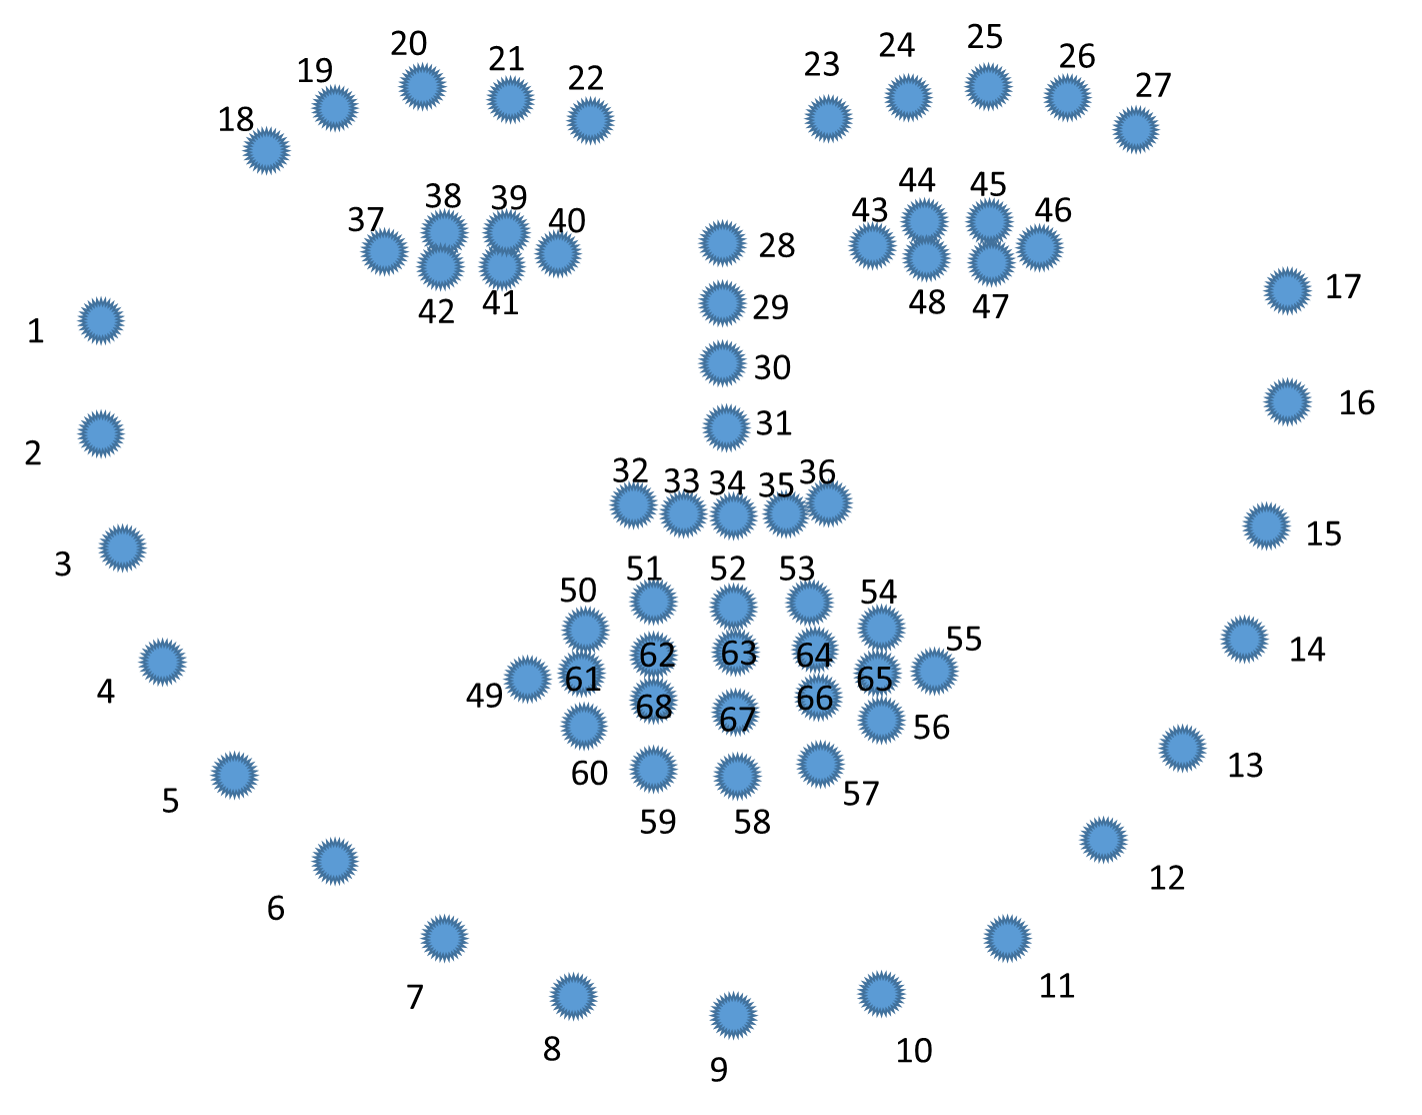
\includegraphics[width=7cm]{./content/materials/enum_landmark.png} }}
    \qquad
    \subfloat[Cột mốc gương mặt được dùng làm chuẩn $l_{standard}$]{{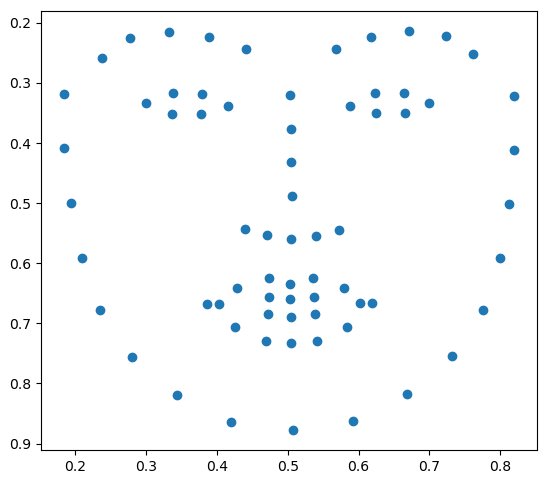
\includegraphics[width=7cm]{./content/materials/standard_landmark.png} }}
    \caption{Xử lý cột mốc gương mặt}
    \label{fig:standard_landmark}
\end{figure}

Tuy nhiên, video đôi khi được quay từ rất nhiều góc độ khác nhau của khuôn mặt, nên việc chuẩn hóa trở nên khó khăn hơn. Vì vậy, ngoài bước xử lý dời điểm 37 và 46, ta cần thêm một số bước xử lý sau để chuẩn hóa cột mốc gương mặt:
\begin{enumerate}
    \item Tính toán cột mốc gương mặt trung bình $l_{avg}$ của tất cả các cột mốc trong video
    \item Để giữ được tỉ lệ của khuôn mặt gốc, ta tính toán một phép biến đổi tương tự (Similarity Transformation) $t_{landmark}$ để chuyển những điểm cột mốc từ số 28 đến số 48 trên cột mốc trung bình $l_{avg}$ thành các điểm tương ứng trên cột mốc chuẩn $l_{standard}$
    \item Áp dụng phép biến đổi $t_{landmark}$ cho từng cột mốc gương mặt riêng lẻ trong video để tạo ra chuỗi cột mốc gương mặt mới đã được điều chỉnh $l_{mod}$
    \item Tìm trong $l_{mod}$ một cột mốc gương mặt có độ mở miệng (khoảng cách giữa điểm 63 và điểm 67) gần với cột mốc gương mặt chuẩn nhất, gọi cột mốc gương mặt đó là $l_{pivot}$
    \item Tìm độ sai lệch $l_{mod-diff}$ của tất cả các cột mốc gương mặt trong $l_{mod}$ so với cột mốc $l_{pivot}$: $l_{mod-diff} = l_{mod} - l_{pivot}$, sau đó tính tổng tích lũy $l_{cumsum}$ của $l_{mod-diff}$. Ta sử dụng cách này như một phương pháp để tách lấy chuyển động tương đối của cột mốc gương mặt ở thời điểm $t$ so với $l_{pivot}$ và bỏ đi các chi tiết đặc trưng của từng gương mặt khác nhau. Tiếp theo, ta cần phải chuyển tất cả các chuyển động này lên $l_{standard}$.
    \item Tìm một phép biến đổi Affine $t_{pivot}$ để chuyển $l_{pivot}$ thành $l_{standard}$. Tuy nhiên ta sẽ không sử dụng trực tiếp ma trận này mà sẽ chỉ sử dụng các hệ số của nó để tính toán ra hệ số phóng đại $s_x$ và $s_y$ tương ứng với từng sự sai lệch ở trục $x$ và $y$ của cột mốc gương mặt trong $l_{cumsum}$ so với cột mốc gương mặt chuẩn $l_{standard}$. Hai số $s_x$ và $s_y$ được gộp lại vào ma trận $s$.
    \item Áp dụng hệ số phóng đại $s$ lên lên tất cả các cột mốc gương mặt trong $l_{cumsum}$, kết quả của phép chuyển đổi này cho biết sự sai lệch của cột mốc gương mặt chuẩn $l_{standard}$ so với cột mốc gương mặt được chuẩn hóa. Như vậy, để tìm ra cột mốc gương mặt được chuẩn hóa $l_{final}$, ta áp dụng công thức: $l_{final} = l_{standard} + l_{cumsum}*s$
    \item Cột mốc gương mặt sau khi xử lý vẫn còn bị ảnh hưởng bởi việc di chuyển đầu. Vì vậy, ta tiếp tục làm thêm một bước chuẩn hóa đơn giản để kéo phần mũi và miệng vào vị trí trung tâm trong khung hình. Theo đó, biến đổi Affine tiếp tục được sử dụng để dịch chuyển các điểm 28, 31, 34, 52, 58, 9 từ $l_{final}$ về các điểm tương ứng trên $l_{standard}$.
\end{enumerate}

Hình sau cho thấy hiệu quả của phép biến đổi trên. Cột mốc gương mặt gốc (màu xanh) bị biến dạng mạnh so với cột mốc chuẩn. Tuy nhiên qua phép biến đổi, ta đã phần nào khôi phục và xấp xỉ được hình dạng của cột mốc gương mặt nếu nhìn thẳng, đồng thời loại bỏ hoàn toàn đặc trưng khuôn mặt của cá nhân người nói. Cột mốc gương mặt này sẽ được dùng để huấn luyện mạng.

\begin{figure}[H]
    \centering
    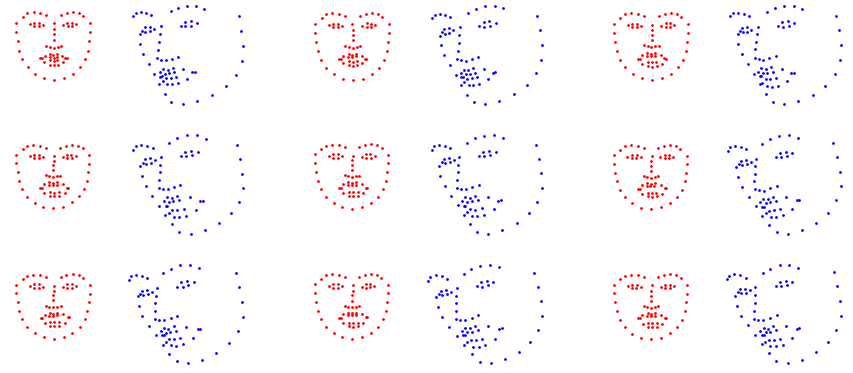
\includegraphics[width=15cm]{./content/materials/standardize_landmark.png}
    \caption{Kết quả chuẩn hóa cột mốc gương mặt. Đỏ - sau chuẩn hóa, xanh - cột mốc gương mặt gốc}
\end{figure}

Sau khi có được cột mốc gương mặt được chuẩn hóa $l_{final}$, ta tiến hành chuẩn hóa hình ảnh khuôn mặt để chuẩn bị dữ liệu hình ảnh cho việc huấn luyện. Hình ảnh mặt người cần được cắt ra từ video gốc là một khung hình vuông, có kích thước 128x128 điểm ảnh quay trực tiếp vào mặt người đang nói. Khung hình phải đảm bảo chứa tất cả các thành phần của khuôn mặt. Khuôn mặt được chuẩn hóa dựa trên việc biến đổi của các thành phần trên cột mốc gương mặt ở bước chuẩn hóa trước. Qua đó, ta so sánh sự biến đổi từ cột mốc gương mặt sau khi được chuẩn hóa vùng mắt với cột mốc chuẩn $l_{standard}$. Trên mỗi video, đối với từng khung hình, ta lần lượt tìm biến đổi Affine để chuyển các điểm cột mốc 28, 31, 34, 49, 55 từ cột mốc gương mặt ban đầu thành cột mốc chuẩn $l_{standard}$. Ta sử dụng ma trận biến đổi này để áp dụng lên khung hình thô của video, nhằm tạo ra một góc nhìn khác nhau cho từng khung hình mà tại đó gương mặt ít bị biến đổi trong quá trình di chuyển và ăn khớp nhất với cột mốc chuẩn. Sau khi hình được biến đổi, ta sử dụng thư viện Dlib để cắt ảnh gương mặt từ trong khung hình này. Những khung hình này là những khung hình đã được chuẩn hóa và sẽ được đem đi huấn luyện mạng. Kết quả xử lý hình ảnh theo phương pháp trên được thể hiện ở hình sau.

\begin{figure}[H]
    \centering
    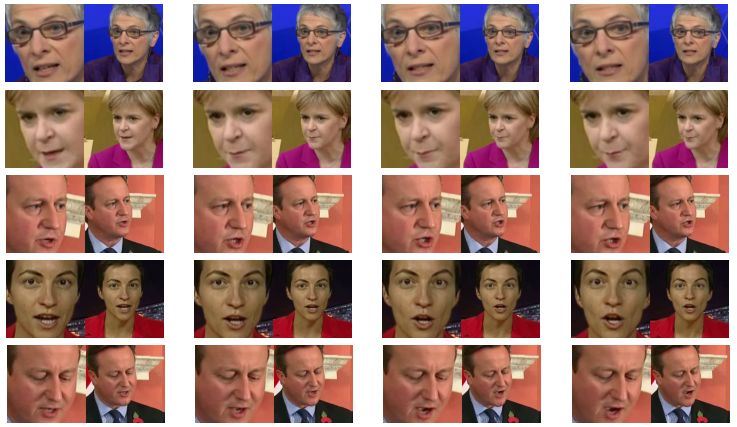
\includegraphics[width=15cm]{./content/materials/preprocess-image.png}
    \caption{Kết quả chuẩn hóa hình ảnh. Có 20 cập hình, ở mỗi cặp hình thì hình bên phải là khung hình gốc, hình bên trái là gương mặt đã được cắt sau khi áp dụng phép biến đổi Affine}
\end{figure}


\section{Cấu trúc chi tiết của hệ thống}

Hệ thống tạo sinh hình ảnh được lấy ý tưởng từ bài báo \cite{chen2019} và được chia làm ba phần:
\begin{itemize}
    \item \textbf{Mạng giải mã cột mốc gương mặt (Landmark Decoder):} Mạng giải mã cột mốc gương mặt là một mạng nơ ron nhận đầu vào là đặc trưng MFCC của giọng nói và cột gốc gương mặt của khung hình mẫu. Như đã nói ở phần \ref{sec:modeling}, ta sẽ không sử dụng trực tiếp đặc trưng âm thanh ở phần mạng GANs vì nó không "gần" với đặc trưng hình ảnh. Vì vậy, mạng giải mã cột mốc gương mặt được dùng để tạo ra cột mốc gương mặt tương ứng với giọng nói trong âm thanh đã cho nhằm mục đích cung cấp một đặc trưng tốt hơn và gần hơn với hình ảnh gương mặt cần được tạo sinh.
    \item \textbf{Mạng tạo sinh hình ảnh (Generator):} Mạng tạo sinh hình ảnh với đầu vào là hình ảnh mẫu của người muốn tạo sinh, cột mốc gương mặt của ảnh và chuỗi cột mốc gương mặt được dự đoán bởi mạng giải mã cột mốc gương mặt. Đầu ra của mạng là chuỗi hình ảnh được tạo sinh hoàn chỉnh của gương mặt người đang nói. Mạng tạo sinh có chức năng trích xuất và tổng hợp các đặc trưng từ đầu vào, kết hợp chung với nhau theo trục không gian và thời gian để tạo ra hình ảnh chân thật và mượt mà nhất. Đây cũng là phần tạo sinh của mạng GANs được dùng trong bài
    \item \textbf{Mạng phân biệt hình ảnh (Discriminator):} Mạng phân biệt hình ảnh có đầu vào là chuỗi hình ảnh trong video gốc hoặc chuỗi hình ảnh được tạo sinh từ mạng tạo sinh, kèm theo đó là cột mốc gương mặt của hình mẫu. Đầu ra của mạng là điểm số xác suất dự đoán liệu chuỗi hình ảnh được đưa vào mạng có phải là chuỗi hình ảnh được trích xuất từ video thật hay chỉ là ảnh được tạo sinh bởi mạng tạo sinh. Ngoài ra mạng cũng cố gắng dự đoán cột mốc gương mặt trong chuỗi hình ảnh được đưa vào mạng nhằm mục đích tạo ra chuyển động khớp với video gốc hơn. Mạng phân biệt này kết hợp với mạng tạo sinh ở trên để tạo thành hệ thống mạng GANs.
\end{itemize}

\subsection{Cấu trúc của bộ giải mã cột mốc gương mặt (Landmark Decoder)}

Bộ giải mã cột mốc gương mặt là một mạng học sâu được ghép nối từ nhiều mạng nhỏ khác nhau, bao gồm mạng tích chập để rút trích đặc trưng MFCC (MFCC Encoder), mạng LSTM, và các mạng kết nối đầy đủ để chuyển các đặc trưng ở lớp cuối thành đầu ra cho mạng.

\begin{figure}[H]
    \centering
    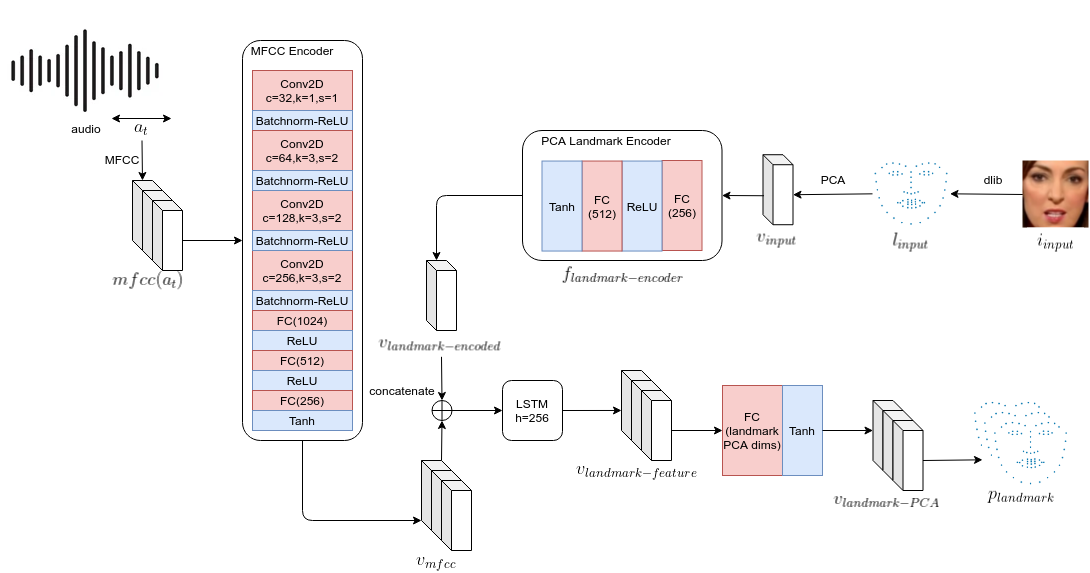
\includegraphics[width=15cm]{./content/materials/landmark_decoder.png}
    \caption{Cấu trúc của bộ giải mã cột mốc gương mặt (Landmark Decoder)}
\end{figure}

Cấu trúc chi tiết của mạng được thể hiện ở hình trên. Như đã nói ở trên, âm thanh được trích xuất MFCC với cửa sổ 10ms, mỗi khung hình có thời lượng là 40ms (do video được thu ở tốc độ ghi hình 25FPS), do đó, tensor MFCC của 1 khung hình có kích thước 1x12x4. Tuy nhiên, để tạo ra được cột mốc gương mặt cho 1 khung hình, ta cần phải lấy đặc trưng MFCC của 3 khung hình trước nó, 3 khung hình sau nó và cả chính nó. Vậy, tổng cộng ta cần dùng đặc trưng âm thanh từ 7 khung hình. Như vậy, tensor MFCC để tạo sinh ra một khung hình có kích thước 1x12x28, vầ đây chính là kích thước của $mfcc(a_t)$. Mạng MFCC Encoder có chức năng trích xuất đặc trưng từ tensor $mfcc(a_t)$ bằng phương pháp tích chập. Mạng có 4 lớp tích chập, 4 lớp Batchnorm và 4 lớp kích hoạt ReLU để trích xuất các đặc trưng ban đầu. Các lớp kết nối đầy đủ ở cuối mạng được dùng để học các đặc trưng bậc cao và tạo ra véc tơ đầu ra có kích thước 256 chiều $v_{mfcc}(t)$. Với $N$ khung hình ở đầu vào, ta sẽ có được $N-6$ véc tơ tạo thành chuỗi véc tơ 256 chiều $v_{mfcc}$ do 3 khung hình đầu và 3 khung hình cuối không được sử dụng. Như vậy, tensor $v_{mfcc}$ có kích thước 256x(N-6)

Cột mốc trong ảnh mẫu sau khi được chuẩn hóa sẽ được thu gọn số chiều nhờ vào giải thuật PCA. Mục đích của việc sử dụng PCA ở đây là để loại bỏ các tác động từ chuyển động đầu của người nói. PCA Landmark Encoder là bộ trích xuất đặc trưng dùng các lớp kết nối đầy đủ nhằm trích xuất đặc trưng của đầu vào $v_{input}$ nhằm tạo ra véc tơ $v_{landmark-encoded}$ có chiều dài 512. Véc tơ $v_{landmark-encoded}$ được nối nối tiếp với từng véc tơ $v_{mfcc}(t)$ nhằm kết hợp đặc trưng cột mốc với đặc trưng âm thanh. Tại mỗi thời điểm $t$, đặc trưng này là một véc tơ có kích thước 768 chiều. Như vậy, sau khi kết hợp hai đặc trưng này lại bằng cách nối tiếp các véc tơ, ta sẽ có chưỡi véc tơ đặc trưng $v_{landmark-feature}$ có kích thước (N-6)x768. Mỗi véc tơ $v_{landmark-feature}(t)$ được đưa vào mạng LSTM theo thứ tự thời gian. Mạng LSTM là mạng có kích thước ẩn là 256. Vì vậy, với mỗi véc tơ $v_{landmark-feature}(t)$ được đưa vào mạng, ta sẽ có được một véc tơ đầu ra có chiều dài 256. Véc tơ đầu ra này được đưa vào mạng kết nối đầy đủ, với đầu ra là số chiều bằng với số chiều được dùng để lấy PCA cho $l_{input}$, với hàm kích hoạt là hàm Tanh để cho ra $v_{landmark-PCA}$. Với mỗi véc tơ $v_{landmark-PCA}(t)$, ta áp dụng phép lấy PCA ngược để tạo ra chuỗi cột mốc gương mặt $p_{landmark}$, và đây chính là chuỗi cột mốc gương mặt được dự đoán cho âm thanh ở đầu vào.

Tóm lại, mạng giải mã cột mốc được mô hình hóa bằng công thức toán như sau:

\begin{equation}
    \begin{split}
    v_{landmark-encoded} &= f_{landmark-encoder}(PCA(l_{input}))\\
    v_{mfcc}(t) &= f_{mfcc-encoder}(mfcc(a_t))\\
    v_{landmark-feature} &= LSTM(v_{landmark-encoded} \oplus v_{mfcc})\\
    p_{landmark} &= PCA_R(\varphi_{landmark}(v_{landmark-feature}))
    \end{split}
\end{equation}

Mạng giải mã cột mốc gương mặt (Landmark Decoder) được huấn luyện độc lập với các mạng còn lại do dữ liệu đã sẵn có ở đầu vào và đầu ra, cũng như để đơn giản hóa quá trình huấn luyện. Đầu ra của mạng là chuỗi các cột mốc gương mặt sẽ được dùng như đầu vào cho mạng GANs tạo sinh ảnh sẽ được nói đến trong phần tiếp theo. Mạng này được huấn luyện với hàm mất mát MSE truyền thống. Gọi $l_{original}$ là chuỗi cột mốc gương mặt được trích xuất từ đoạn video có chứa âm thanh được đưa vào đầu vào của mạng, hàm mất mát của mạng được biểu diễn như sau:

\begin{equation}
    \mathcal{L}_{landmark} = \frac{1}{n}\sum^n_{i=1}(l_{original}-p_{landmark})^2
\end{equation}

\subsection{Cấu trúc của bộ tạo sinh hình ảnh (Generator)}\label{sec:generator_detail}

Bộ tạo sinh hình ảnh là phần quan trọng nhất trong hệ thống. Bộ tạo sinh hình ảnh (Generator) là phần tạo sinh dữ liệu trong hệ thống mạng GANs. Bộ tạo sinh hình ảnh nhận đầu vào là hình ảnh mặt người mẫu $i_{input}$, cột mốc gương mặt được trích xuất từ ảnh người mẫu $l_{input}$ và chuỗi cột mốc gương mặt được dự đoán từ âm thanh được sinh ra bởi mạng giải mã cột mốc gương mặt (Landmark Decoder). Hình ảnh người mẫu $i_{input}$ đã được chuẩn hóa các điểm ảnh sao cho giá trị của tất cả các điểm ảnh trên tất cả các kênh màu nằm trong khoảng [-1, 1], tương tự, các cột mốc gương mặt $l_{input}$ và $p_{landmark}$ đều được đưa về khoảng [-0.5, 0.5]. Đầu ra của mạng, như đã nói ở phần \ref{sec:modeling} gồm có 3 chuỗi hình ảnh có độ dài bằng nhau: $p_{att}$ là mặt nạ chú ý, cho ta biết những vùng nào trên gương mặt trong ảnh gốc cần được chỉnh sửa, $p'_{image}$ là ảnh được tạo sinh có hình dạng mặt người nhưng không được hoàn hảo, cho ta biết ta nên thay đổi hình ảnh gốc như thế nào. Và cuối cùng là chuỗi hình ảnh được tạo sinh, là sự kết hợp giữa hình ảnh gốc $i_{input}$ và ảnh tạo sinh $p'_{image}$ ở từng điểm ảnh với trọng số được quyết định bởi $p_{att}$ 

\begin{figure}[H]
    \centering
    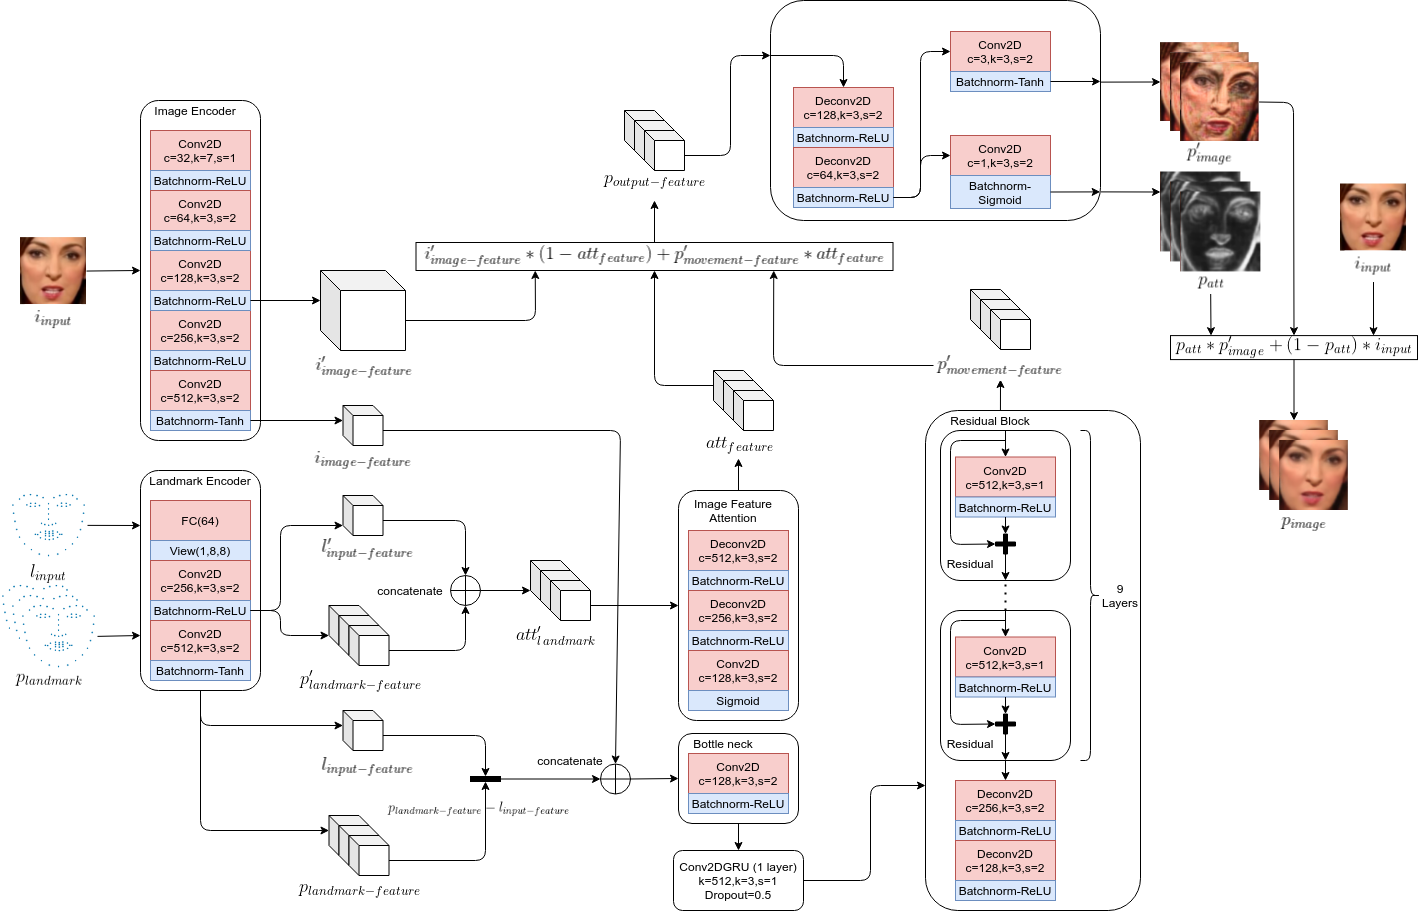
\includegraphics[width=15cm]{./content/materials/generator.png}
    \caption{Cấu trúc của bộ giải mã landmark của khuôn mặt (Generator)}
\end{figure}

Hình ảnh mẫu $i_{input}$ được trích xuất đặc trưng bằng mạng Image Encoder gồm 5 lớp tích chập để tạo thành tensor đặc trưng $i_{image-feature}$. Mạng Landmark Encoder cũng được sử dụng để trích xuất đặc trưng từ cột mốc gương mặt. Tại thời điểm này, các cột mốc gương mặt là một ma trận 68x2 (68 điểm cột mốc ở hai trục $(x,y)$). Ma trận này được duỗi thẳng thành véc tơ 136 chiều và đưa vào mạng Landmark Encoder để trích xuất đặc trưng. Mạng Landmark Encoder ở đầu có một lớp kết nối đầy đủ, chuyển véc tơ 136 chiều thành véc tơ 64 chiều. Véc tơ 64 chiều sau đó được chuyển dạng thành tensor có kích thước 1x8x8. Tensor này đi qua hai lớp tích chập để đưa ra tensor đặc trưng $l_{input-fearure}$ là đặc trưng được trích xuất từ $l_{input}$ và chuỗi tensor đặc trưng $p_{landmark-feature}$ được trích xuất từ chuỗi cột mốc $p_{landmark}$. Sau đó, theo chiều thời gian, các tensor trong chuỗi $p_{landmark-feature}$ được trừ cho $l_{input-feature}$, việc trừ các tensor này cho nhau nhằm mục đích trích xuất các đặc trưng khác biệt giữa cột mốc mẫu và các cột mốc được tạo sinh và từ đó cho thấy sự chuyển động của các điểm trên gương mặt. Lúc này, $i_{image-feature}$ và các tensor kết quả của phép trừ vừa thực hiện đều có kích thước 512x8x8, ta tiến hành nối tiếp $i_{image-feature}$ với các tensor trên theo chiều channel. Như vậy, ta sẽ tạo ra được các tensor đặc trưng cho mỗi khung hình có kích thước 1024x8x8. Tensor đặc trưng này là sự kết hợp bởi tensor chứa đặc trưng hình ảnh và tensor chứa đặc trưng chuyển động của các cột mốc gương mặt theo thời gian, nhờ vậy, ta đã kết hợp được sự chuyển động trên gương mặt được tạo ra bởi âm thanh và hình ảnh ban đầu. Các đặc trưng này là cơ sở để tìm ra sự thay đổi cần phải áp dụng lên hình ảnh gốc để tạo sinh ra hình ảnh tương ứng với cột mốc gương mặt được tạo sinh. Tại đây, mạng Bottle neck được sử dụng để thu nhỏ kích thước các tensor và một mạng hồi quy tích chập được sử dụng để xem xét tính chất thời gian trong chuỗi đặc trưng được đưa vào. Mạng hồi quy tích chập được thiết kế với một lớp hồi quy, sử dụng 512 kênh và nhân tích chập có kích thước bằng 3, đồng thời sử dụng lớp bỏ bớt dữ liệu ở cuối với tỉ lệ bỏ bớt dữ liệu là 50\%. Việc sử dụng một mạng hồi quy tích chập là nhằm mục đích làm cho chuyển động của hình ảnh mượt mà, hợp lý và mang tính thời gian, có trước có sau. Sau khi được thêm vào tính chất thời gian bởi mạng hồi quy tích chập, đặc dữ liệu này tiếp tục được trích xuất đặc trưng bằng mạng Residual Block. Đây là một mạng rất sâu gồm 9 lớp tích chập được nối tắt (Residual) và 2 lớp tích chập ngược. Mục đích của mạng Residual Block là tăng cường thêm nhiều lớp có trọng số học để mạng được sâu hơn, chứa được nhiều thông tin hơn, trích xuất được nhiều đặc trưng có giá trị hơn. Sau khi qua mạng Residual Block, ta có một chuỗi tensor $p'_{movement-feature}$, với mỗi tensor $p'_{movement-feature}(t)$ trong chuỗi là đặc trưng sẽ được dùng để tạo sinh khung hình tại thời điểm $t$.

Quay trở lại với mạng Landmark Encoder, trong quá trình tính toán ra $l_{input-feature}$ và $p_{landmark-feature}$, thì tại khối tích chập - Batchnorm - ReLU đầu tiên, mạng cũng tạo ra các đặc trưng sớm của các cột mốc gương mặt được đưa vào mạng, đó là đặc trưng $l'_{input-feature}$ được tạo ra từ $l_{input}$ và chuỗi đặc trưng $p'_{landmark-feature}$ được tạo ra từ $p_{landmark}$. Với từng tensor $p'_{landmark-feature}(t)$ tại thời điểm $t$, ta ghép nối nó với $l'_{input-feature}$ theo chiều channel để tạo ra chuỗi tensor $att'_{landmark}$. Các tensor trong chuỗi $att'_{landmark}$ chứa thông tin về cột mốc gương mặt mẫu và cột mốc gương mặt tại thời điểm $t$. Thông tin này giúp phần mạng phía sau có thêm thông tin để so sánh và tìm ra những vị trí trên gương mặt có sự thay đổi tại thời điểm $t$ so với ảnh gốc. Ta đưa chuỗi tensor $att'_{landmark}$ vào mạng Image Feature Attention, mạng này gồm 2 lớp tích chập ngược ở đầu và đầu ra là lớp tích chập với hàm kích hoạt Sigmoid. Nhờ lớp kích hoạt Sigmoid, mạng Image Feature Attention tạo ra chuỗi tensor $att_{feature}$ với các giá trị trong tensor nằm trong khoảng [0, 1]. 

Lúc này, ta sẽ kết hợp các đặc trưng vừa trích xuất được để tạo ra đặc trưng hình ảnh bậc cao hơn. Chuỗi véc tơ đặc trưng hình ảnh $p_{output-feature}$ được tổng hợp với công thức:
\begin{equation}
    \begin{split}
    p_{output-feature}(t) = &i'_{image-feature}*(1-att_{feature}(t))+\\
    &p'_{movement-feature}(t)*att_{feature}(t)
    \end{split}
\end{equation}

Với $i'_{image-feature}$ là đặc trưng sớm được trích xuất từ ành mẫu $i_{image}$ sau khi qua 3 lớp tích chập đầu tiên của mạng Image Encoder. Như vậy, trong công thức này, $att_{feature}$ hoạt động như một mặt nạ chú ý ở cấp độ tensor. Mặt nạ chú ý $att_{feature}$ có chức năng lọc ra các đặc trưng chuyển động mong muốn từ $p'_{movement-feature}$, phần đặc trưng bị lọc bỏ sẽ được bù vào bởi đặc trưng hình ảnh gốc $i'_{image-feature}$. Với công thức này, chiến lược của hệ thống sẽ là lấy một phần đặc trưng của ảnh gốc, và thay thế một số thành phần trên ảnh gốc bằng các thành phần mô tả chuyển động để tạo ra ảnh mới. Chuỗi đặc trưng $p_{output-feature}$ đi qua thêm 2 lớp tích chập ngược để tăng kích thước chuỗi tensor. Tại điểm này, mỗi tensor đặc trưng cho một hình trong chuỗi có kích thước 64x128x128. Những tensor này chia thành hai hướng, một hướng đi qua mạng tích chập có ngõ ra là 3 kênh, tạo ra hình ảnh $p'_{image}$ với ba kênh màu RGB. Hướng thứ hai, chuỗi tensor đi qua một lớp tích chập có ngõ ra 1 kênh. Với hàm kích hoạt Sigmoid, mạng tích chập này tạo ra hình ảnh mặt nạ chú ý $p_{att}$. Như chiến thuật tạo sinh hình ảnh đã nói ở trên, ta kết hợp hình ảnh ban đầu $i_{image}$ với hai chuỗi hình ảnh vừa tạo ra để tạo thành chuỗi hình ảnh trên video đầu ra $p_{image}$. Tóm lại, mạng tạo sinh được mô hình hóa bằng công thức toán như sau:
\begin{equation}
    \begin{split}
    i'_{image-feature}, i_{image-feature} &= f_{image}(i_{input})\\
    l'_{input-feature}, l_{input-feature} &= f_{landmark}(l_{input})\\
    p'_{landmark-feature}, p_{landmark-feature} &= f_{landmark}(p_{landmark})\\
    p'_{movement-feature}(t) &= f_{residual}(CRNN(f_{bottle}(i_{image-feature} \\
    &\oplus (p_{landmark-feature}(t)-l_{input-feature}))))\\
    att_{feature}(t) &= f_{att}(p'_{landmark-feature}(t) \oplus l'_{input-feature})\\
    p_{output-feature}(t) &= i'_{image-feature}*(1-att_{feature}(t))+\\
    &p'_{movement-feature}(t)*att_{feature}(t)\\
    p_{att}(t), p'_{image}(t) &= f_{out}(p_{output-feature}(t))\\
    p_{image}(t) &= p_{att}(t)*p'_{image}(t)+(1-p_{att}(t))*i_{image}
    \end{split}
\end{equation}

\subsection{Cấu trúc của bộ phân biệt hình ảnh (Discriminator)}\label{sec:discriminator_detail}

Thành phần thứ hai trong hệ thống mạng GANs là mạng phân biệt Discriminator có chức năng phân biệt ảnh thật (hình ảnh được lấy từ video gốc) hay ảnh giả (hình ảnh được tạo sinh bởi mạng Generator). Hàm mất mát của mạng phân biệt được sử dụng để cập nhật trọng số cho chính nó và cho mạng tạo sinh. Đầu vào của mạng phân biệt là chuỗi hình ảnh được dự đoán bới mạng tạo sinh $p_{image}$ hoặc chuỗi hình ảnh thật được lấy ra từ dữ liệu huấn luyện $i_{video}$, kèm theo đó là cột mốc của gương mặt mẫu $l_{input}$. Đầu ra của mạng là nhãn cho chuỗi hình ảnh được đưa vào mạng để dự đoán xem chuỗi hình ảnh được đưa vào là hình ảnh thật hay hình ảnh được tạo sinh, đồng thời, mạng cũng tái tạo lại một chuỗi cột mốc gương mặt $p_{landmark-discriminator}$ tương ứng với chuỗi hình ảnh được đưa vào mạng.

\begin{figure}[H]
    \centering
    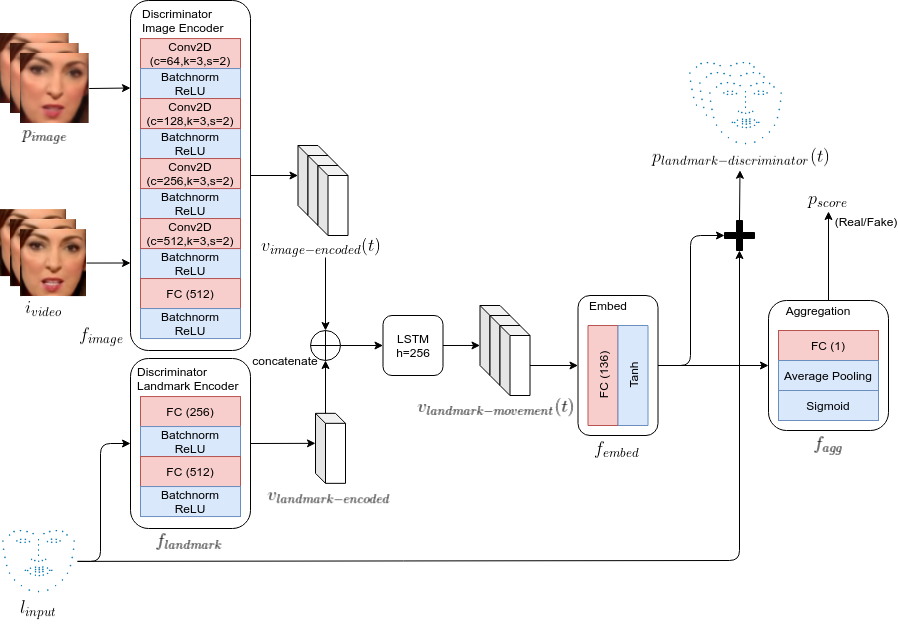
\includegraphics[width=15cm]{./content/materials/discriminator.png}
    \caption{Cấu trúc của bộ phân biệt hình ảnh (Discriminator)}
\end{figure}

Cũng như mạng tạo sinh hình ảnh, chuỗi hình ảnh đưa vào mạng được trích xuất đặc trưng bằng mạng Discriminator Image Encoder. Mạng này gồm 4 lớp tích chập và một lớp kết nối đầy đủ để biến đổi đặc trưng được trích xuất thành một véc tơ 512 chiều. Chuỗi hình ảnh trong mạng sau khi được trích xuất đặc trưng sẽ cho ra chuỗi véc tơ $v_{image-encoded}(t)$ là các véc tơ 512 chiều được sắp xếp theo thứ tự thời gian. Cột mốc gương mặt $l_{input}$ trích xuất từ hình mẫu cũng được đưa vào mạng. $l_{input}$ được duỗi thẳng thành véc tơ 136 chiều và được đưa vào mạng Discriminator Landmark Encoder. Mạng này dùng 2 lớp kết nối đầy đủ để trích xuất đặc trưng từ véc tơ cột mốc gương mặt. Đầu ra của mạng là véc tơ đặc trưng $v_{landmark-encoded}$ 512 chiều. Véc tơ đặc trưng này được ghép nối tiếp với từng véc tơ trong chuỗi $v_{image-encoded}$ để tạo thành chuỗi véc tơ 1024 chiều. Chuỗi véc tơ này được đưa qua mạng LSTM với kích thước lớp ẩn là 256 để trích xuất đặc trưng thời gian, đầu ra của mạng LSTM là chuỗi véc tơ 256 chiều $v_{landmark-movement}$. Chuỗi véc tơ này chứa đặc trưng chuyển động của ảnh theo thời gian và liên kết chuyển động đó với hình dạng cột mốc gương mặt của người mẫu. Một lớp kết nối đầy đủ với hàm kích hoạt Tanh được sử dụng để cho ra một chuỗi véc tơ 136 chiều, đây chính là chuỗi véc tơ mô tả chuyển động của cột mốc gương mặt người nói theo thời gian. Ta lần lượt cộng các chuyển động này vào cột mốc gương mặt mẫu $l_{input}$ để tìm ra được chuỗi cột mốc gương mặt $p_{landmark-discriminator}(t)$ được dự đoán cho chuỗi hình ảnh được đưa vào. Cũng trên chuỗi véc tơ chuyển động $v_{landmark-movement}$, ta cho qua mạng Aggregation bao gồm 1 lớp kết nối đầy đủ có kích thước đầu ra bằng 1 để biến đổi số chiều của véc tơ 136 chiều về 1 chiều, sau đó ta dùng lớp lấy mẫu trung bình (Average Pooling) để tính trung bình cộng theo thời gian và qua hàm kích hoạt Sigmoid để tìm ra xác suất để đánh nhãn chuỗi hình ảnh đưa vào mạng là thật hay giả. Mạng phân biệt được biễu diễn dưới dạng công thức toán như sau:
\begin{equation}
    \begin{split}
    v_{image-encoded}(t) &= f_{image}(p_{image}(t)|i_{video}(t))\\
    v_{landmark-encoded} &= f_{landmark}(l_{input})\\
    v_{landmark-movement} &= LSTM(v_{image-encoded} \oplus v_{landmark-encoded})\\
    p_{landmark-discriminator}(t) &= f_{embed}(v_{landmark-movement}(t) + l_{input})\\
    p_{score} &= f_{agg}(f_{embed}(v_{landmark-movement}))
    \end{split}
\end{equation}

\subsection{Hàm mất mát được sử dụng cho hệ thống mạng GANs}

Từ cấu trúc chung của hệ thống được thể hiện ở hình \ref{fig:common_architecture}, ta có thể thấy, mạng GANs được sử dụng có hai nhánh hàm mất mát: hàm mất mát cho từng điểm ảnh và hàm mất mát GANs. Hàm mất mát cho từng điểm ảnh được sử dụng với mục đích huấn luyện cho mạng cách tạo ra hình ảnh giống với hình ảnh thật nhất. Như ta thấy trên hình \ref{fig:common_architecture}, mặt nạ chú ý $p_{att}$ tập trung vào những điểm có liên quan đến sự chuyển động của khuôn mặt theo âm thanh (như mắt, miệng, cằm), và bỏ qua các điểm không liên quan (tóc, mũi, phông nền,...). Như vậy, ta sẽ chú ý nhiều hơn đến những điểm được thay đổi trên khuôn mặt để cố gắng làm cho nó giống nhất với video thật. Dựa trên ý tưởng này, hàm mất mát cho từng điểm ảnh tại mạng tạo sinh có công thức:

\begin{equation}
    \mathcal{L}_{pix} = \frac{1}{T}\sum^T_{t=1}||(i_{video}(t)-p_{image}(t))*(p_{att}(t)+\beta)||_1
\end{equation}

Trong đó:
\begin{itemize}
    \item \textbf{$i_{video}(t)$}: khung hình tại thời điểm $t$ của video gốc
    \item \textbf{$p_{image}(t)$}: hình ảnh được tạo sinh tại thời điểm $t$
    \item \textbf{$p_{att}(t)$}: mặt nạ chú ý được dự đoán tại thời điểm $t$
    \item \textbf{$\beta$}: một hằng số để đảm bảo tất cả các điểm trên ảnh đều được học, ta chọn $\beta = 0.5$ 
\end{itemize}

Hàm mất mát GANs trong mạng được thiết kế nhằm mục đích cố gắng làm cho hình ảnh tạo sinh khó phân biệt với hình ảnh thật nhất có thể, đồng thời cũng tạo ra những chuyển động gương mặt tương đồng với chuyển động trong video thật. Việc tạo ra hình ảnh chân thật, khó phân biệt với ảnh gốc được đảm bảo bởi hàm mất mát phân biệt sau:
\begin{equation}
    \begin{split}
    \mathcal{L}_{gans-dis} = &\mathbb{E}_{l_{input},i_{video}}[logD_s(l_{input},i_{video})]\\
    +&\mathbb{E}_{l_{input},i_{input},p_{landmark}}[log(1-D_s(l_{input},G(l_{input},i_{input},p_{landmark})))]
    \end{split}
\end{equation}

Trong đó:
\begin{itemize}
    \item \textbf{$l_{input},i_{input},p_{landmark},i_{video}$}: đã được giải thích ở các phần trên
    \item \textbf{$D_s$}: Mạng phân biệt với đầu ra là xác suất ảnh là ảnh thật, đã được miêu tả ở phần \ref{sec:discriminator_detail}
    \item \textbf{$G$}: Mạng tạo sinh hình ảnh được miêu tả ở phần \ref{sec:generator_detail}
\end{itemize}

Nhằm tạo ra các chuyển động gương mặt bám sát với video gốc, mạng phân biệt cũng cố gắng tái tạo lại cột mốc gương mặt rong video gốc. Hàm mất mát GANs theo cột mốc gương mặt được mô tả theo công thức sau:
\begin{equation}
    \begin{split}
    \mathcal{L}_{gans-landmark} = &||(D_l(l_{input},G(l_{input},i_{input},p_{landmark})) - l_{orig})*M_l||^2_2\\
    +&||(D_l(l_{input},i_{video}) - l_{orig})*M_l||^2_2\\
    \end{split}
\end{equation}

Trong đó:
\begin{itemize}
    \item \textbf{$l_{input},i_{input},p_{landmark},i_{video}$}: đã được giải thích ở các phần trên
    \item \textbf{$D_l$}: Mạng phân biệt với đầu ra là cột mốc gương mặt trên ảnh được tạo sinh, đã được miêu tả ở phần \ref{sec:discriminator_detail}
    \item \textbf{$G$}: Mạng tạo sinh hình ảnh được miêu tả ở phần \ref{sec:generator_detail}
    \item \textbf{$l_{orig}$}: Cột mốc gương mặt được trích xuất nguyên gốc từ video $i_{video}$
    \item \textbf{$M_l$}: mặt nạ nhằm chú ý nhiều hơn vào cột mốc gương mặt vùng miệng, theo đó, sai số của cột mốc ở vùng miệng có hệ số 100, trong khi các vùng khác là 1.
\end{itemize}

Cuối cùng, các hàm mất mát trên được kết hợp để cho ra hàm mục tiêu cuối cùng. Công thức của hàm mục tiêu được biểu diễn như sau:
\begin{equation}
    \begin{split}
    \mathcal{L}_{gans} = &\mathcal{L}_{gans-dis} + \mathcal{L}_{gans-landmark}\\
    \mathcal{L} = &\mathcal{L}_{gans} + \lambda*\mathcal{L}_{pix}
    \end{split}
\end{equation}

Theo đó, giá trị mất mát $\mathcal{L}_{pix}$ tại mạng tạo sinh được kết hợp với giá trị mất mát GANs tại mạng phân biệt $\mathcal{L}_{gans}$ để tạo ra giá trị mất mát cuối cùng $\mathcal{L}$. Mục tiêu của quá trình học là giảm tối thiểu giá trị này. Hệ số cân bằng $\lambda$ cũng được sử dụng nhằm mục đích cân bằng giữa $\mathcal{L}_{pix}$ và $\mathcal{L}_{gans}$, ta chọn giá trị này bằng 10.
